\let\textcircled=\pgftextcircled
\chapter{Combined search for the invisible decay of the Higgs boson in hadronic channels}
\label{chap:higgstoinv}

\initial{T}his is the analysis chapter on \higgstoinv.

%=======
\begin{easylist}[itemize]
\ListProperties(Style*=-- , FinalMark={)}, Margin=0.5cm)
& Discuss how the theoretical aspects from the Theory chapter translate into an experimental search.

& Discuss the necessity of including all production modes of Higgs (invisible final state, so characterise events based on initial/additional particles). Also mention how sensitive each production mode is at contributing to the branching ratio limit. Emphasise the non-VBF modes (\ggF, \ttH, \VH\ -- \WplusH, \WminusH, \ZH) in this chapter as that's what I've been working on and another student will be covering \acrshort{vbf}.

& Talk about what makes this analysis unique: doing a combination over all production modes from the start instead of separate analyses combined at the end. Means we can share samples, systematics, background methods and workflows, build in orthogonality between the different modes and cover as much phase space as possible (with new final states such as boosted \PZ bosons with unresolved subjets). This makes the analysis much more cohesive and consistent.

& Include object definitions, overall analysis strategy, triggers, signal production (with each non-VBF mode in detail), event selection, background estimation and results/limit (including comparisons to previous results).

& Emphasise my contributions: control region construction and studies, background estimation, and other studies I will have conducted by the time I write up.

& Current material: no public plots as of yet. Hope to finish analysis by the time I begin writing up. We are preparing a CMS internal analysis note, documenting all aspects of the analysis. I will add all relevant information there which I can subsequently use when writing this chapter.
\end{easylist}


\section{Analysis overview}
\label{sec:htoinv_overview}

\subsection{Hadronic production modes of the Higgs boson}
\label{subsec:htoinv_production_modes}

\begin{figure}[htbp]
    \centering
    \begin{subfigure}[b]{0.5\textwidth}
        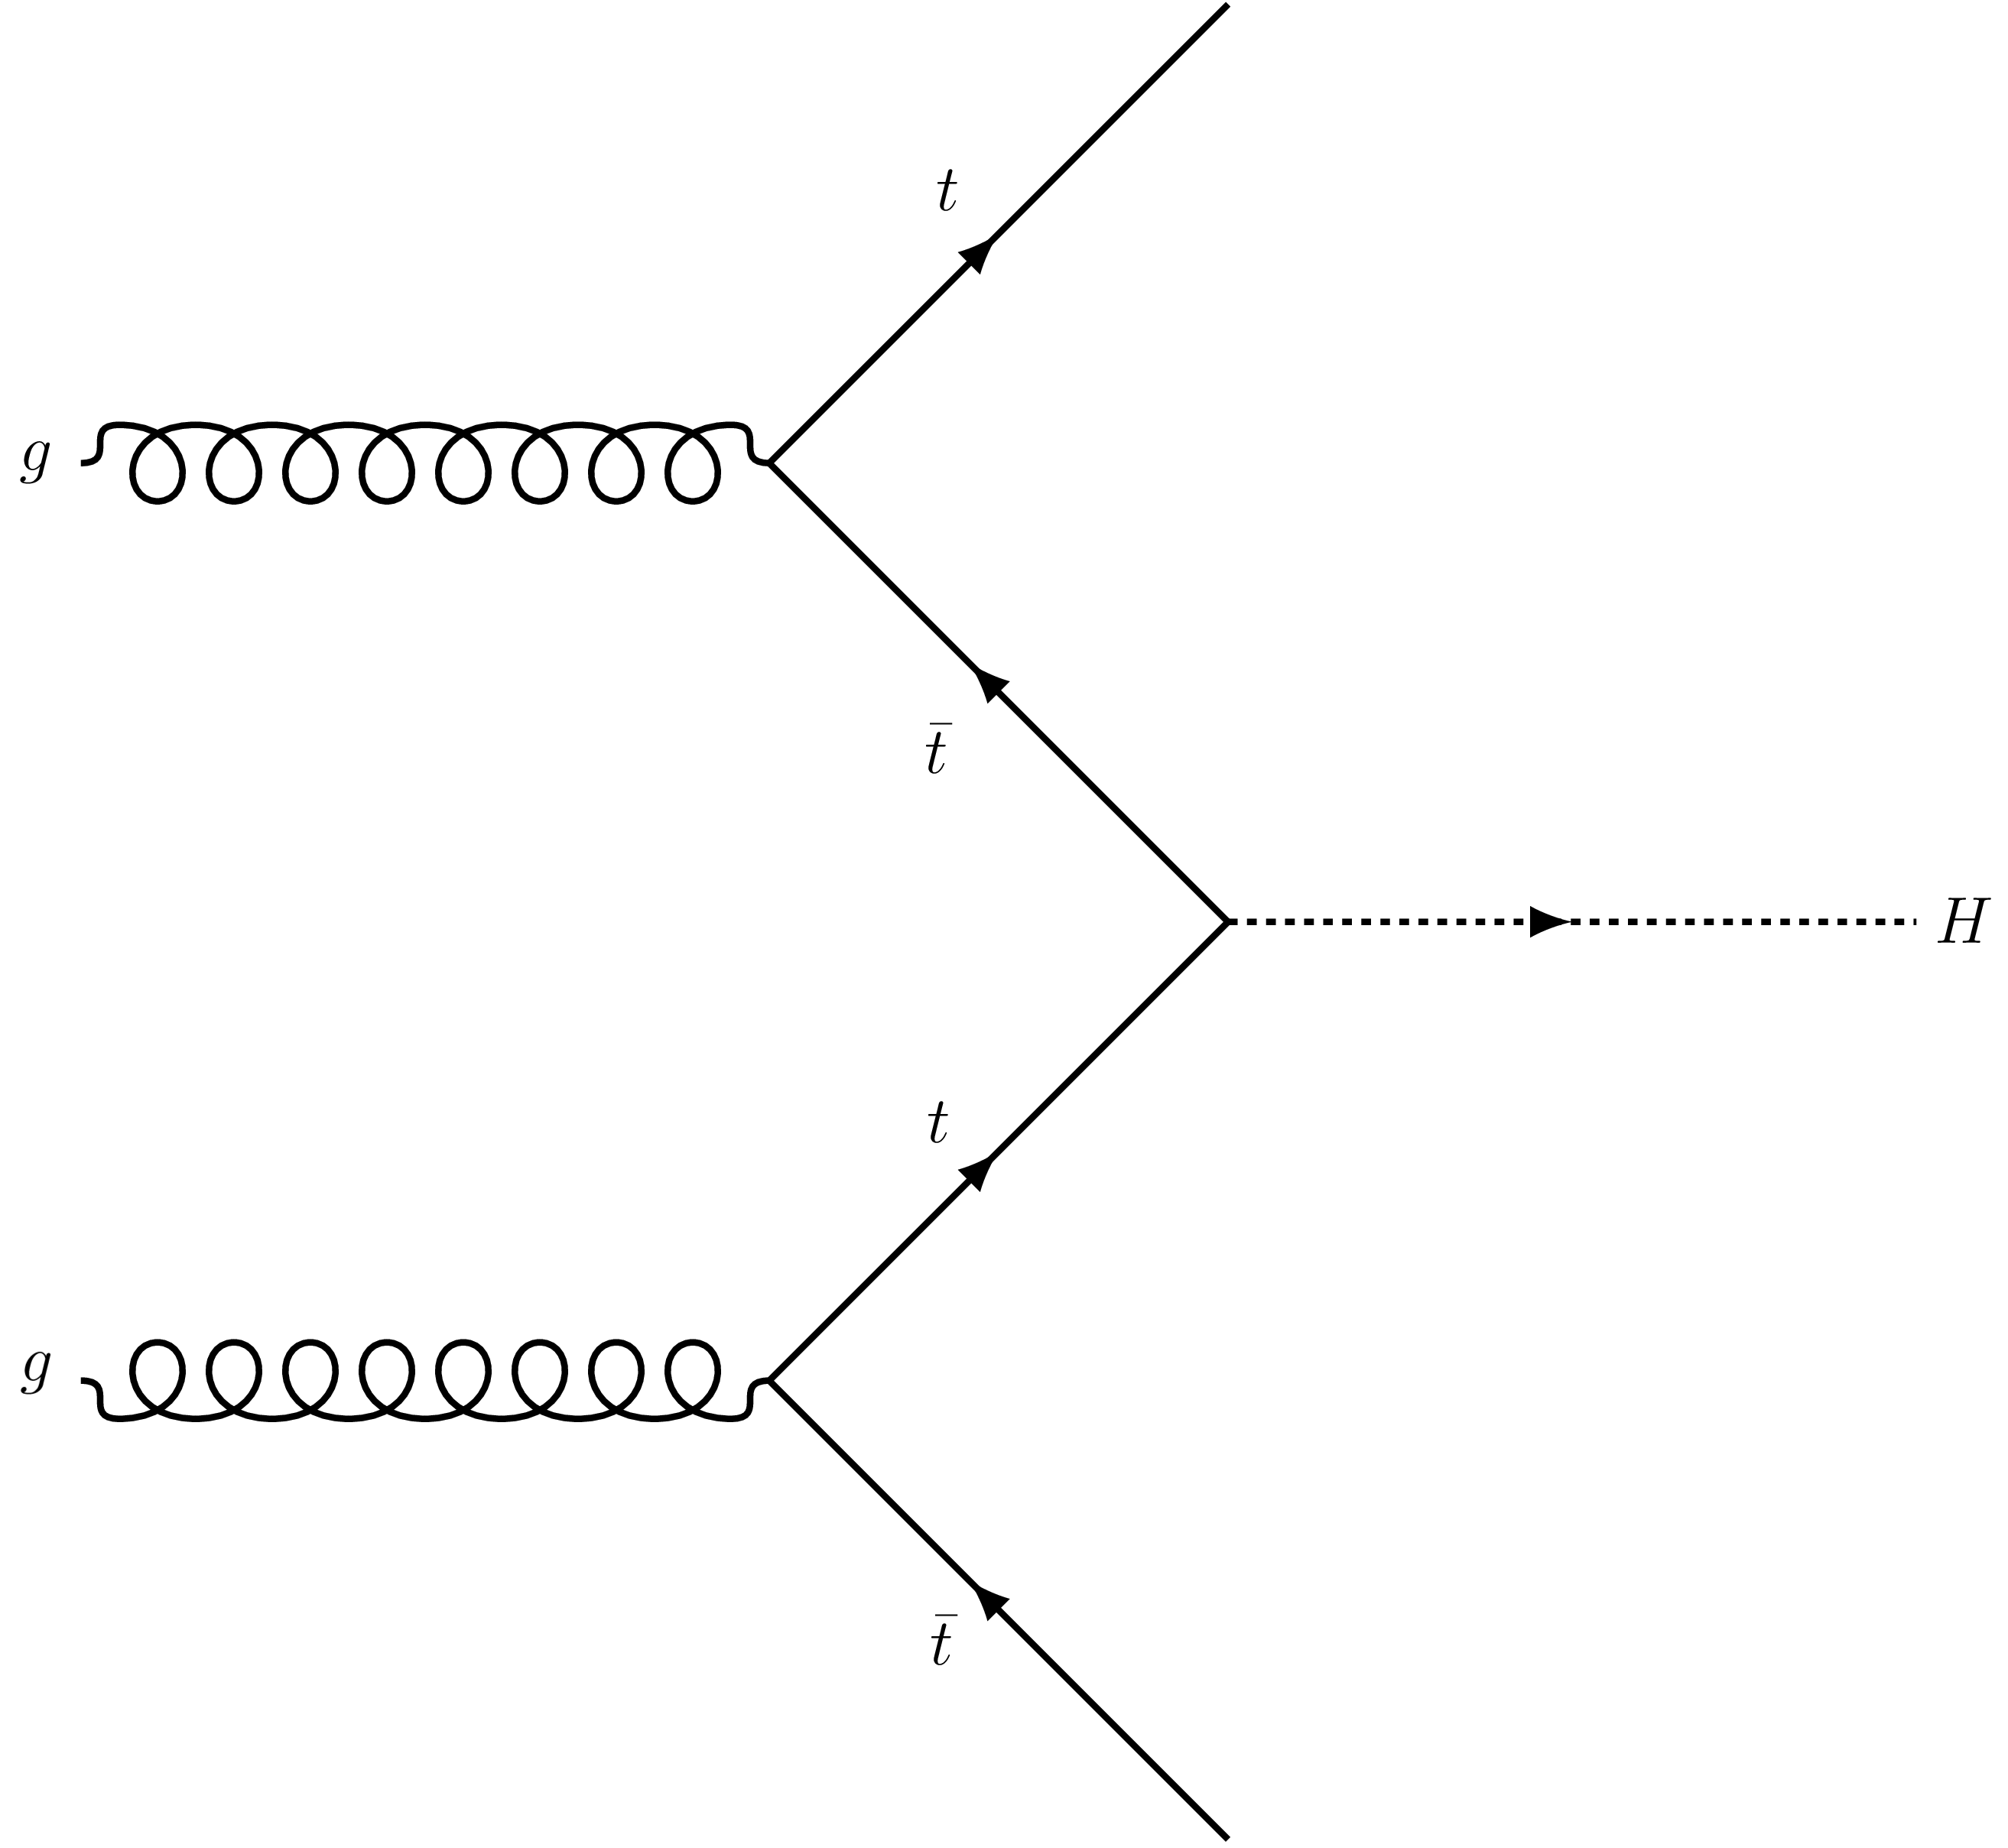
\includegraphics[width=\textwidth]{feynman_diagrams/ttH.png}
        \caption{\ttH}
    \end{subfigure}
    \hfill
    \begin{subfigure}[b]{0.45\textwidth}
        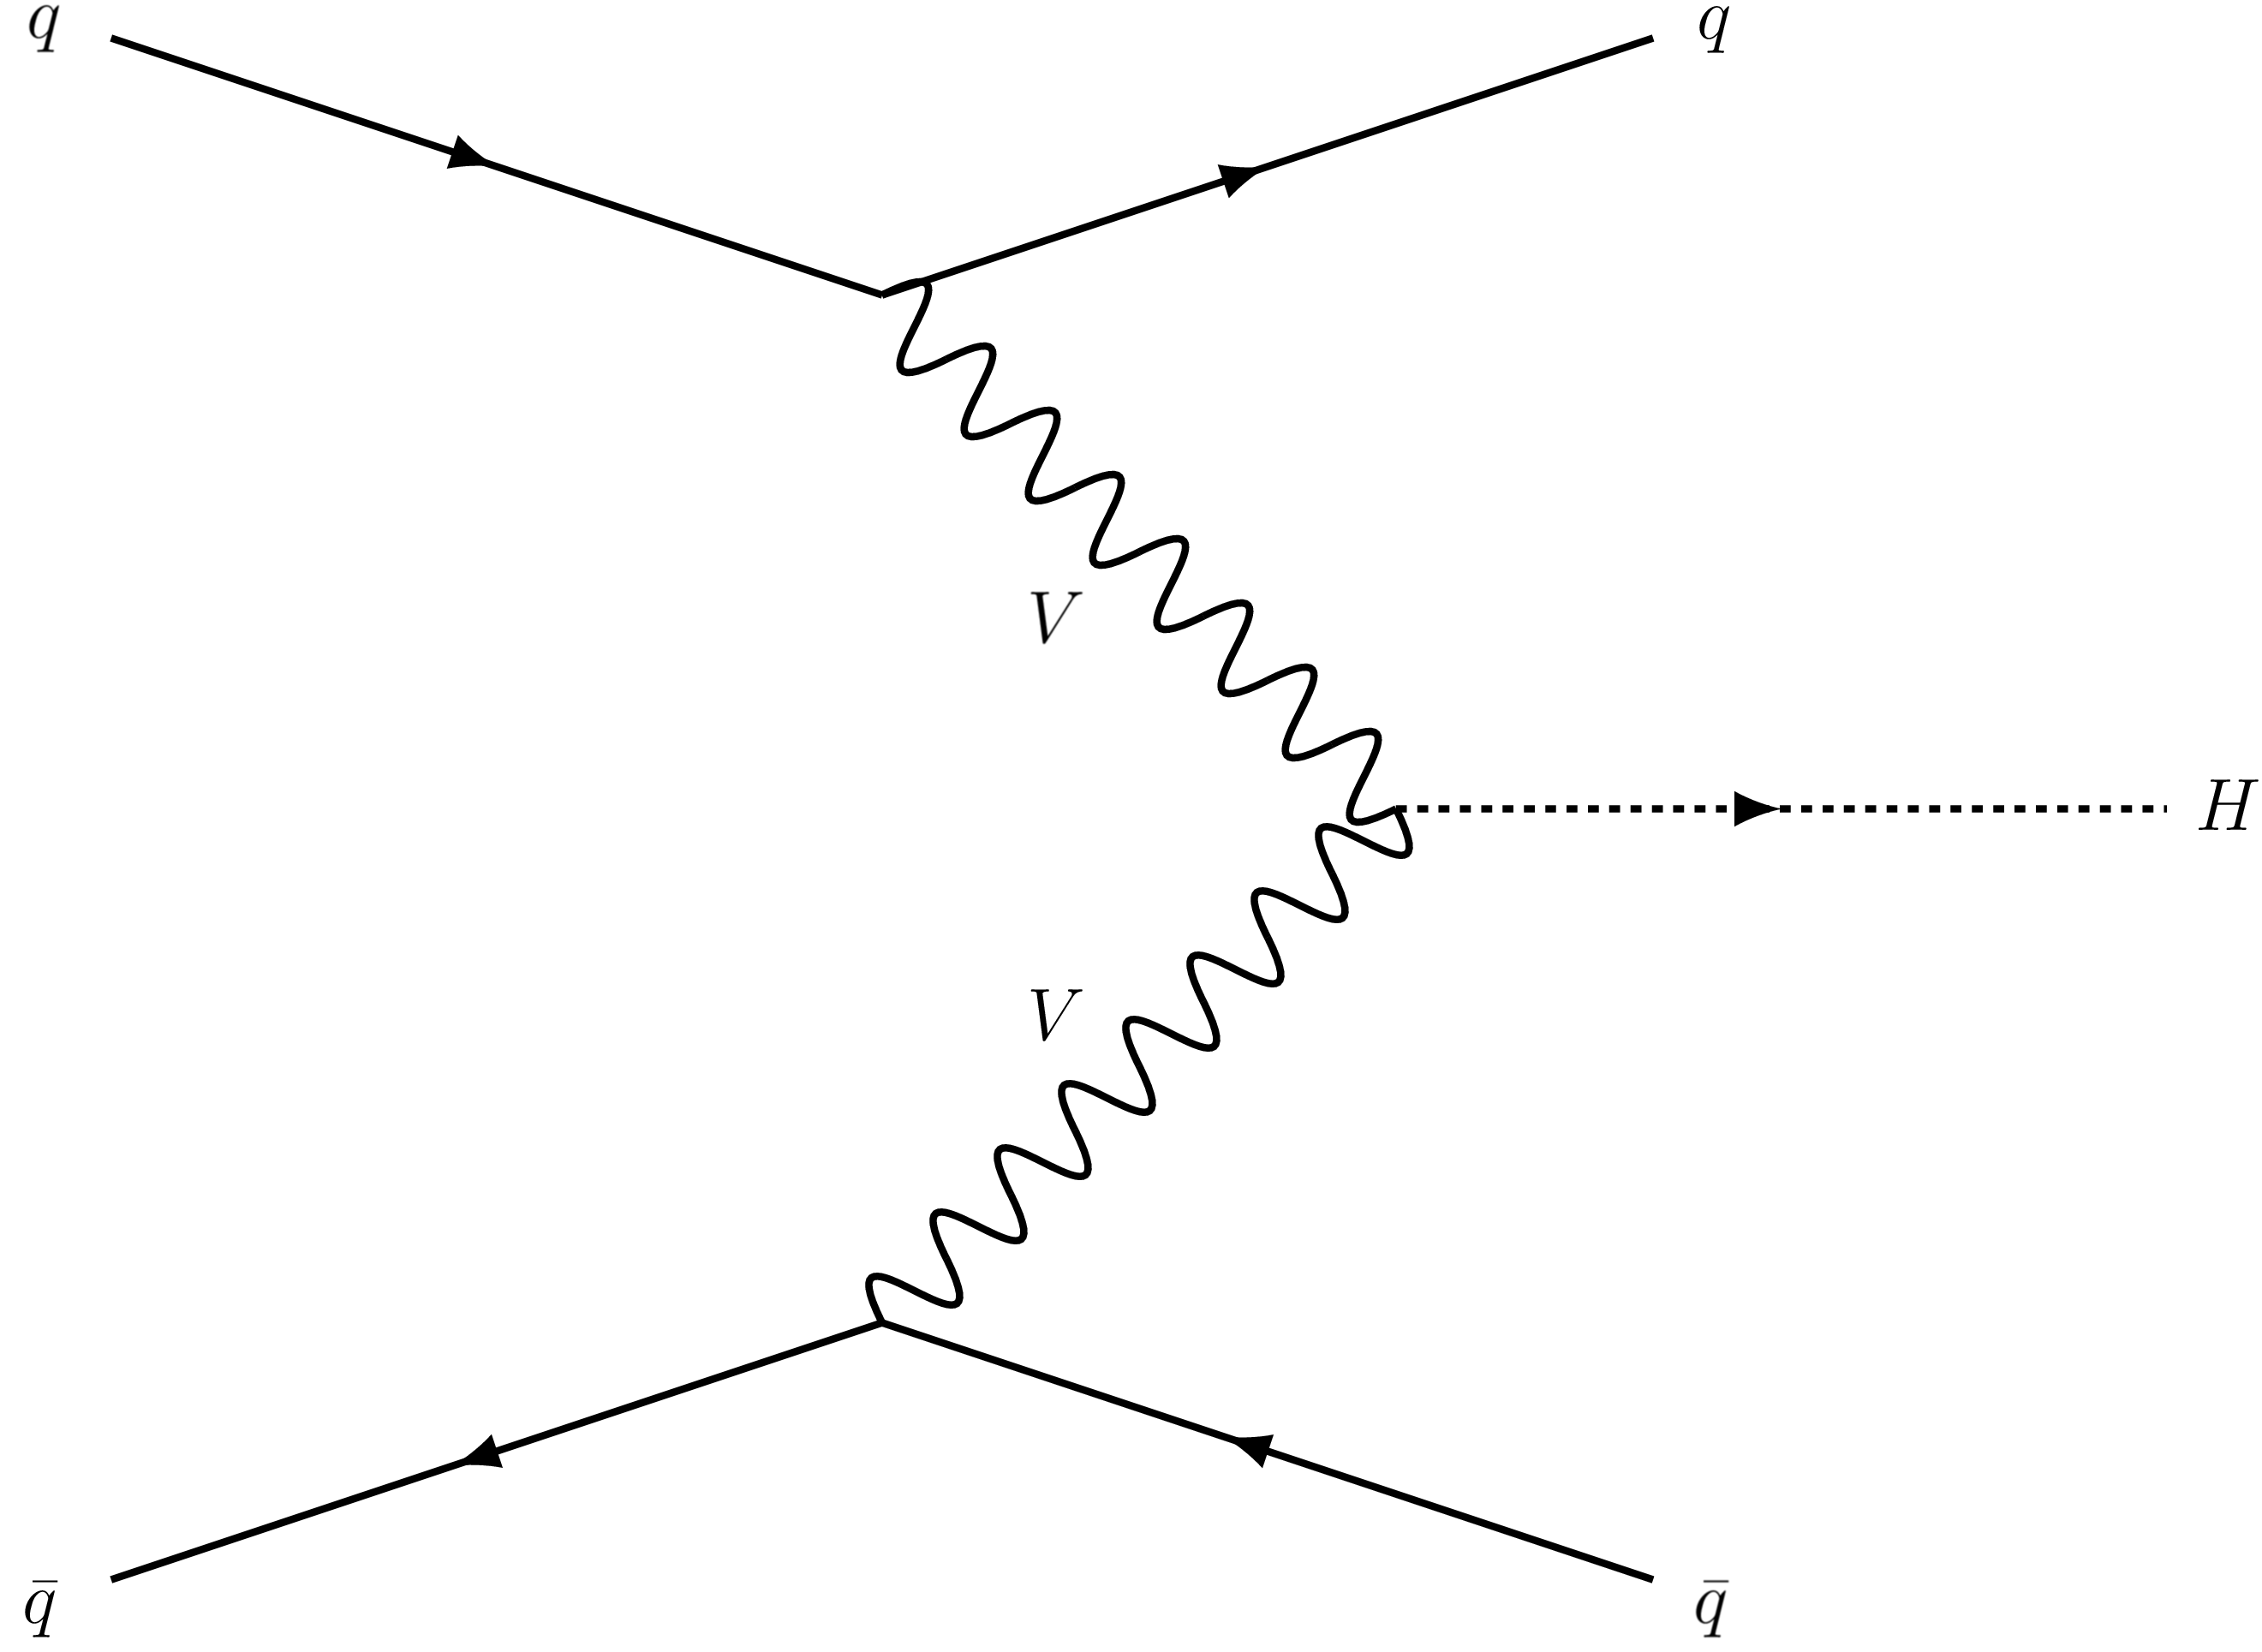
\includegraphics[width=\textwidth]{feynman_diagrams/VBF.png}
        \caption{VBF}
    \end{subfigure}
% blank line to start new row
    \begin{subfigure}[b]{0.45\textwidth}
        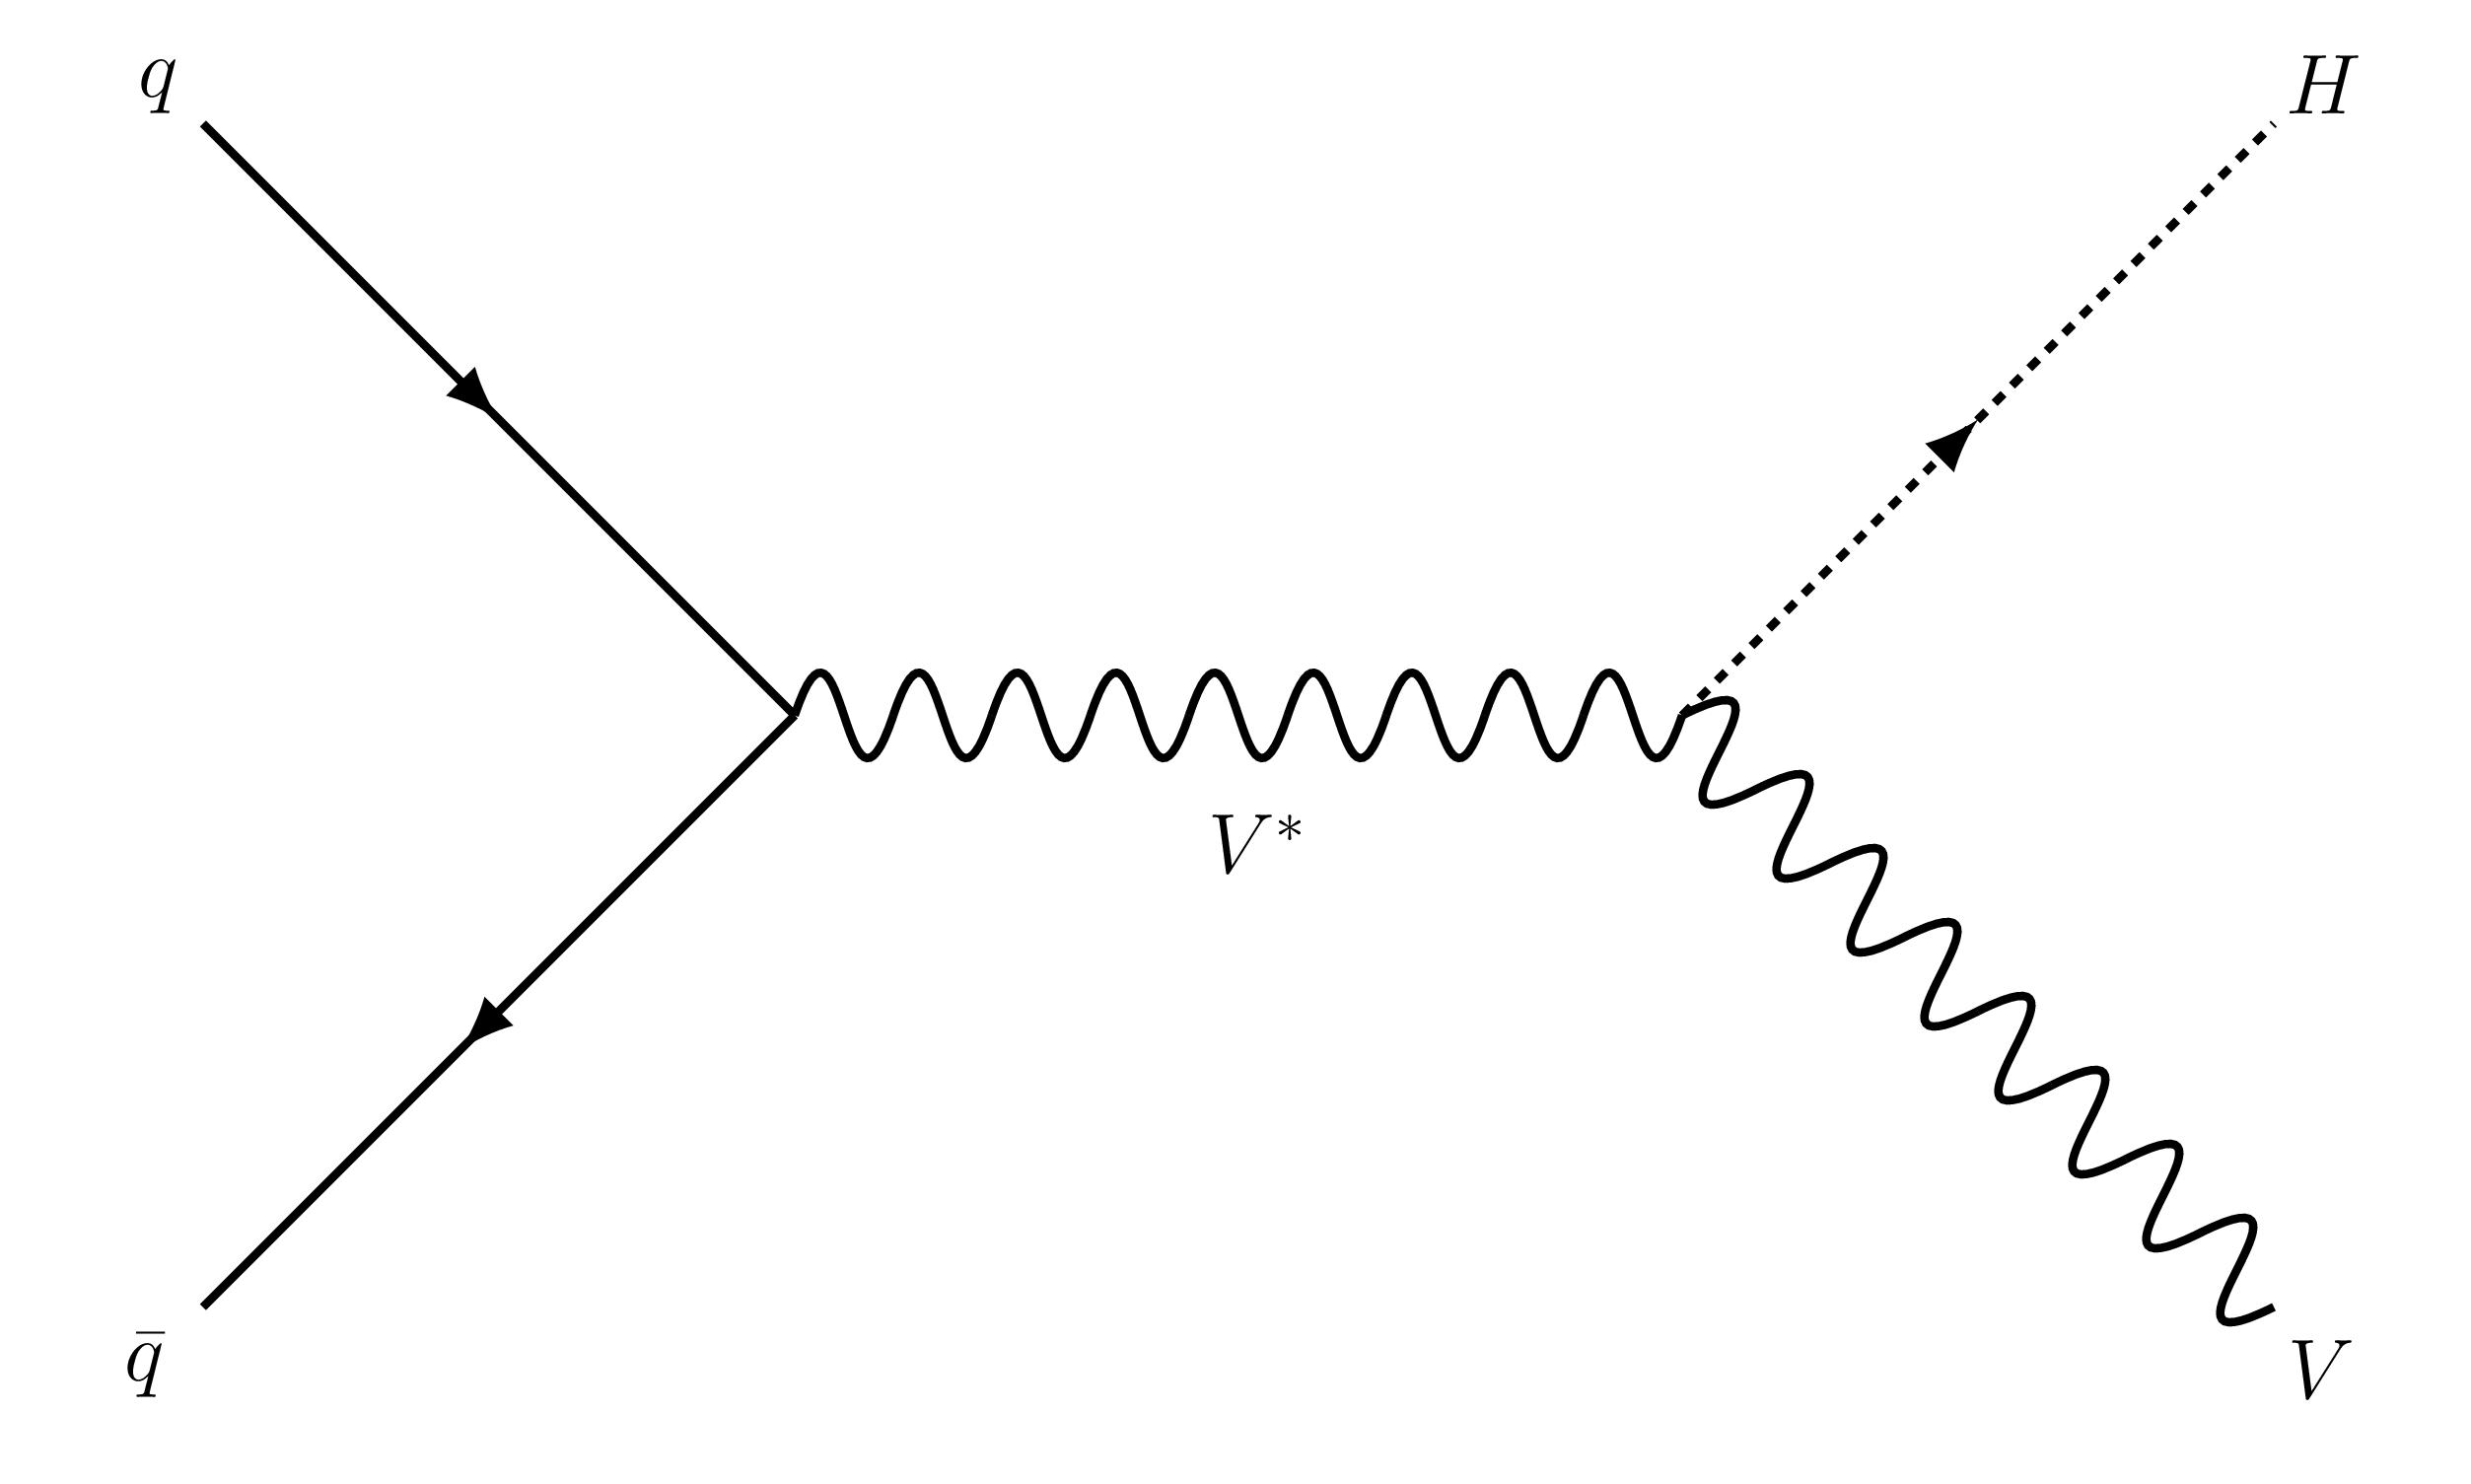
\includegraphics[width=\textwidth]{feynman_diagrams/VH.png}
        \caption{\VH}
    \end{subfigure}
    \hfill
    \begin{subfigure}[b]{0.45\textwidth}
        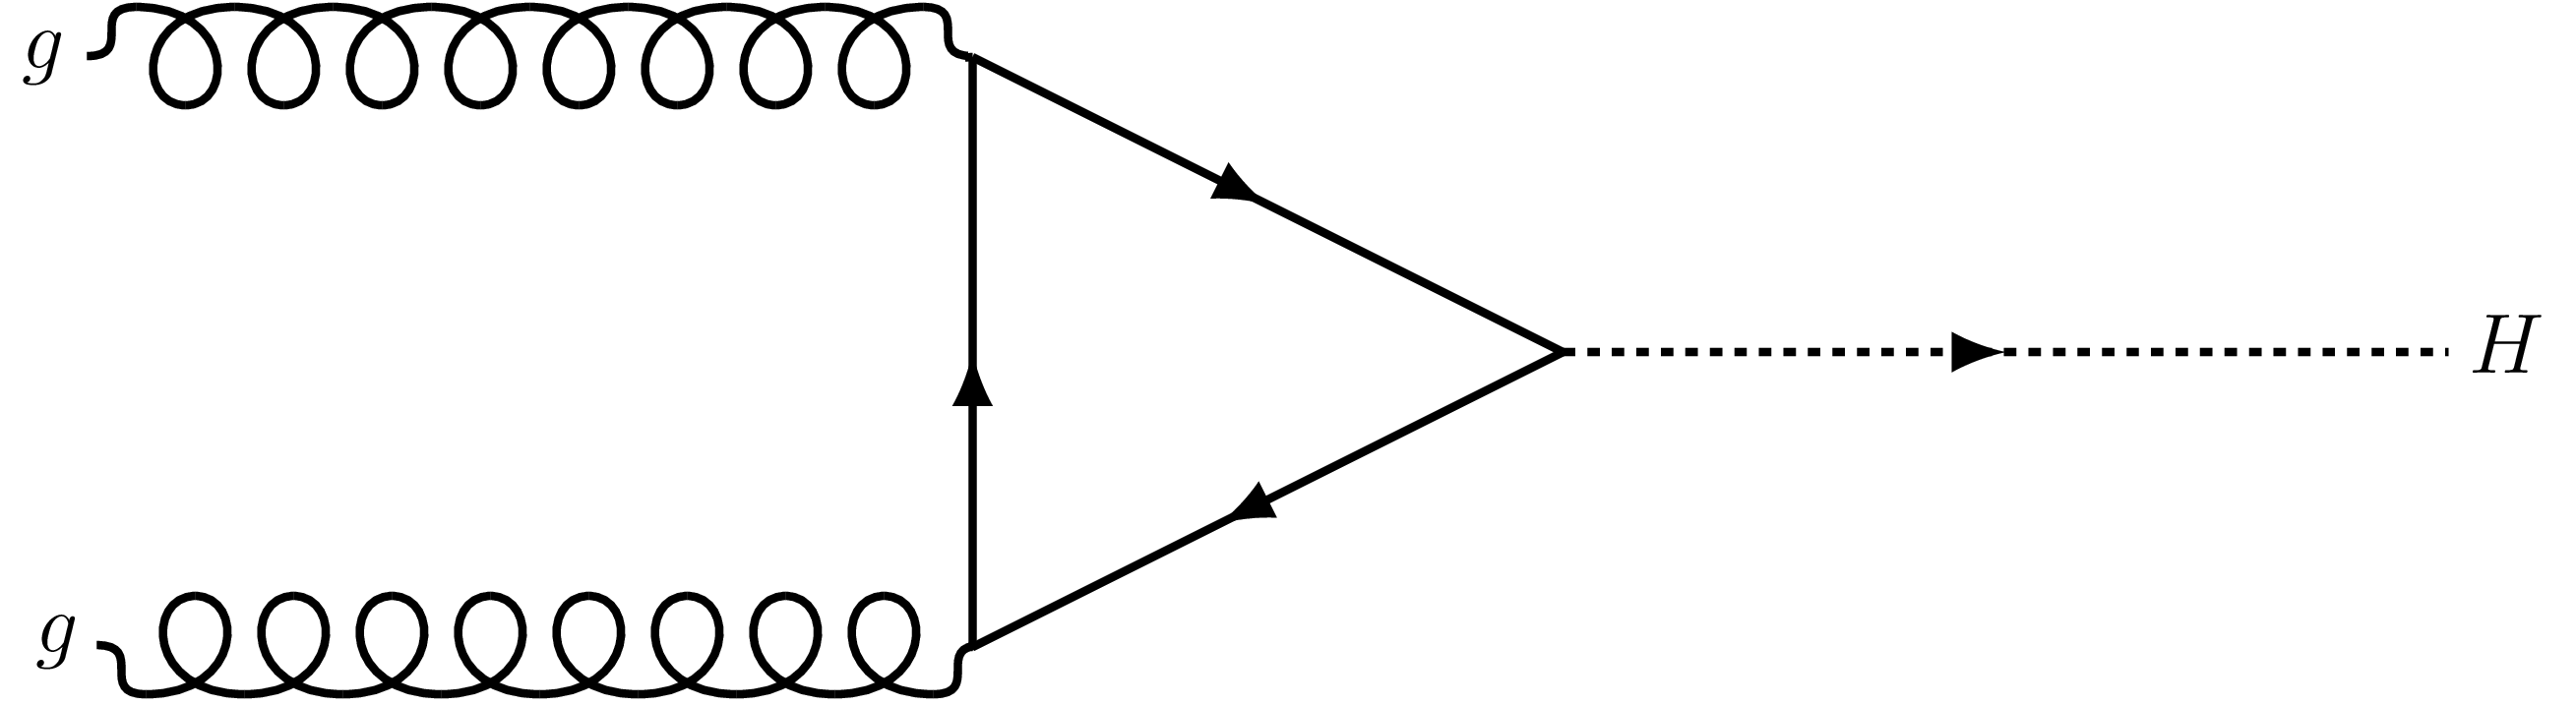
\includegraphics[width=\textwidth]{feynman_diagrams/ggF.png}
        \caption{\ggF}
    \end{subfigure}
\caption{The Feynman diagrams for the four main hadronic production modes of the Higgs boson.} % To add a shorter caption for the figure in the List of Figures, add the shorter caption inside square brackets before the main one, i.e., \caption[Reduced caption]{Full caption}
\label{fig:higgs_feynman_diagrams}
\end{figure}

\section{Data and simulation}
\label{sec:htoinv_data_sim}


\section{Triggers}
\label{sec:htoinv_triggers}


\section{Categorisation of the non-VBF production modes}
\label{sec:htoinv_categorisation}


\section{Background estimation}
\label{sec:htoinv_background_est}

\subsection{Control regions}
\label{subsec:htoinv_crs}

\subsection{Background estimation methods}
\label{subsec:htoinv_background_methods}
